This paragraph considers the expression of a simple example in
\ac{IMP} notation.  We use a 1D three-point averaging kernel as a
stand-in for more complicated operations; the \ac{IMP} model can
handle higher dimensions, as well as irregular graph connectivity.

Consider then the three-point operation
\begin{equation}
  \forall_i\colon y_i=f(x_i,x_{i-1},x_{i+1}).
  \label{eq:3ptscalar}
\end{equation}
We illustrate this graphically by depicting the input and output
vectors, stored distributedly over the processing elements (physical
processor or threads) by contiguous blocks, and the three-point
combining operation:

\includegraphics[scale=.12]{graphics/3pt-avg-ab-plain}

The distribution indicated by vertical dotted lines
we call the $\alpha$-distribution, and it corresponds to 
the traditional concept of distributions in parallel programming systems.
The following is a possible declaration:
\begin{verbatim}
IMP_disjoint_blockdistribution
  *blocked = new IMP_disjoint_blockdistribution
    (problem_environment,globalsize);
IMP_object
  *output_vector = new IMP_object( blocked );
\end{verbatim}

Now, we can in fact identify a second distribution that differs from
the traditional notion. We let the $\beta$-distribution be defined as
the mapping from each processor to all of its needed input elements.
The second illustration depicts these two distributions
for one particular process:

\includegraphics[scale=.12]{graphics/3pt-avg-ab}

The $\beta$-distribution, unlike the $\alpha$ one, is not disjoint:
certain elements are assigned to more than one processing element.

To specify the $\beta$-distribution, we introduce more IMP concepts.
First, if $x$~is a distributed object, and $d$ a distribution,
by $x(d)$ we will mean `$x$~distributed with~$d$'. Furthermore, we
will introduce operations on distributions, 
such as left-shifting or right-shifting a distribution,
as is needed for the combining operation.

In programming terms:
\begin{verbatim}
IMP_disjoint_blockdistribution
  *rightshift = new IMP_disjoint_blockdistribution
    (problem_environment,globalsize);
rightshift->operate(">>1"); 
IMP_disjoint_blockdistribution
  *leftshift = new IMP_disjoint_blockdistribution
    (problem_environment,globalsize);
leftshift->operate("<<1");
\end{verbatim}

The \ac{IMP} framework can now express equation~\eqref{eq:3ptscalar}
in terms of distributions. 
Introducing a notation where for instance $d\gg1$ means `$d$~right-shifted by~1',
we write the three-point kernel as
\[ y(d) \leftarrow f\bigl( x(d),x(d\ll1),x(d\gg1) \bigr). \]
Programmatically we now express
a kernel as the combination of a local function, an output vector,
and the beta distribution, expressed as input with shifted distributions:
\begin{verbatim}
IMP_kernel *update_step = 
  new IMP_kernel(step,output_vector,blocked);
IMP_object *input_vector = // defined elsewhere
update_step->localexecutefn = &threepoint_execute;
update_step->add_beta_vector( input_vector );
update_step->add_beta_vector( input_vector,leftshift );
update_step->add_beta_vector( input_vector,rightshift );
queue->add_kernel( step,update_step );
\end{verbatim}

We compared this code\footnote{All sources available
at \url{https://bitbucket.org/VictorEijkhout/imp-demo}.} to manually
produced reference codes.
\begin{figure}[ht]
\leavevmode\hbox{%
  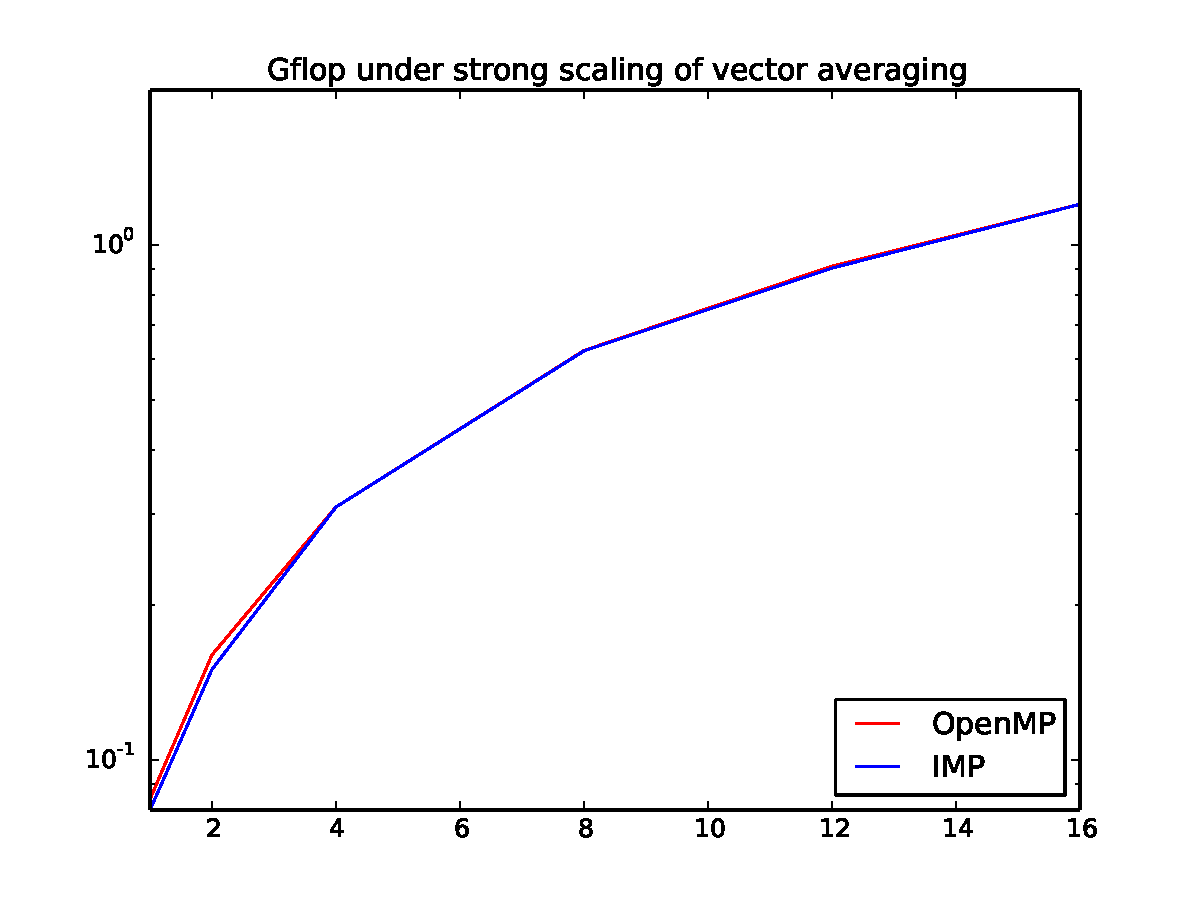
\includegraphics[scale=.4]{graphics/omp_scaling}
  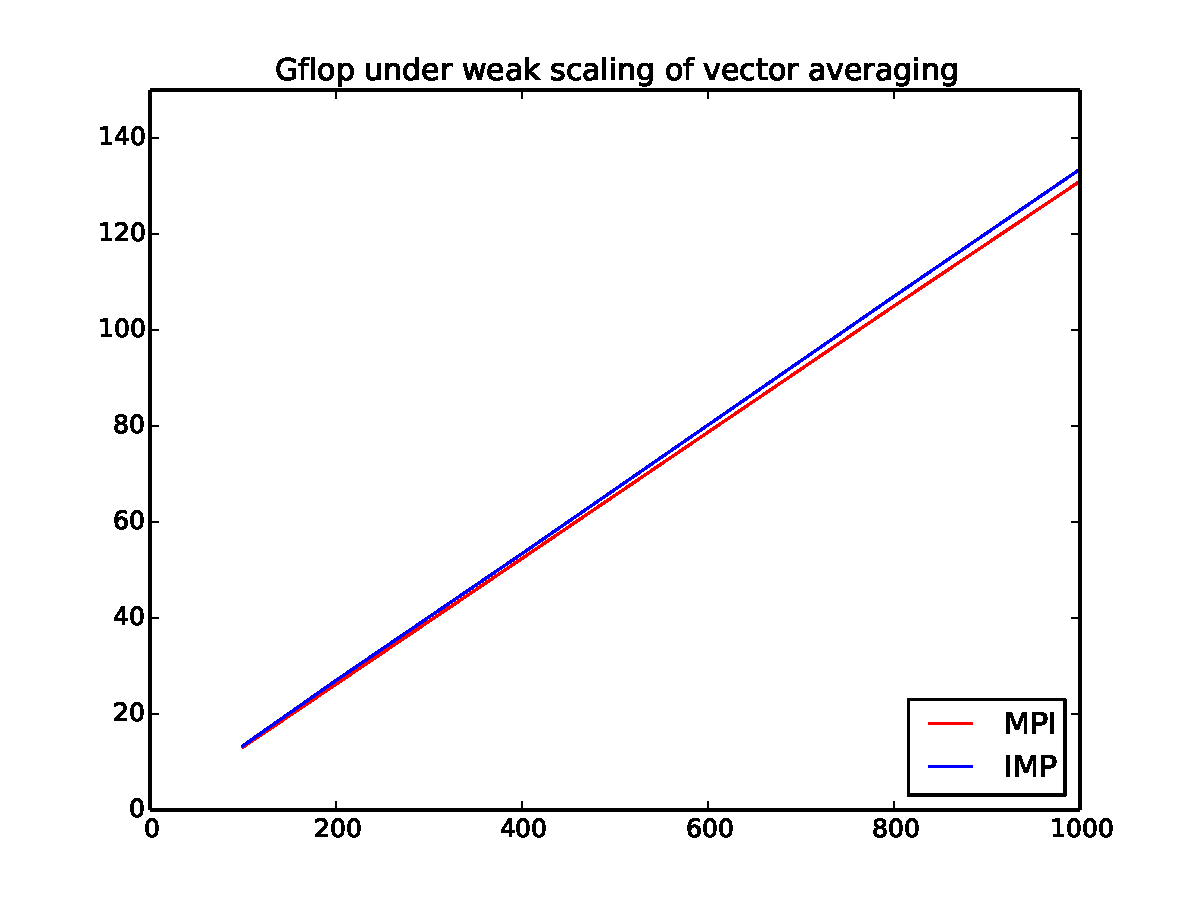
\includegraphics[scale=.4]{graphics/mpi_scaling}
  }
  \caption{Scaling behaviour of OpenMP and MPI realizations of the example IMP code,
  compared to manually produced reference codes.}
  \label{fig:scale}
\end{figure}
Figure~\ref{fig:scale} shows that both with OpenMP and MPI the 
performance behaviour,
possibly after startup phenomena,
is identical within 2--3\%. (On this small example
the line counts of the IMP code and the reference codes
are not appreciably different. We expect
this difference to become more pronounced on
larger codes.)
